   
\documentclass{beamer}
\usepackage{listings}
\lstset{
%language=C,
frame=single, 
breaklines=true,
columns=fullflexible
}
\usepackage{blkarray}
\usepackage{subcaption}
\usepackage{url}
\usepackage{tikz}
\usepackage{tkz-euclide} % loads  TikZ and tkz-base
%\usetkzobj{all}
\usetikzlibrary{calc,math}
\usepackage{float}
\providecommand{\brak}[1]{\ensuremath{\left(#1\right)}}
\providecommand{\pr}[1]{\ensuremath{\Pr\left(#1\right)}}
\newcommand{\myvec}[1]{\ensuremath{\begin{pmatrix}#1\end{pmatrix}}}
\newcommand\norm[1]{\left\lVert#1\right\rVert}
\renewcommand{\vec}[1]{\mathbf{#1}}
\usepackage[export]{adjustbox}
\usepackage[utf8]{inputenc}
\usepackage{amsmath}
\usepackage{tikz}
\usetikzlibrary{automata, positioning}
\usetheme{Boadilla}




\title{Assignment 4 - Linear Forms Q2.35}
\author{Akyam Dhatri Nanda - AI20BTECH11002}
\date{\today }
\begin{document}

\begin{frame}
\titlepage
\end{frame}

\begin{frame}
\frametitle{Question}
\begin{block}{Linear Forms Q2.35}
Find the shortest distance between the lines
\begin{align}
\label{eq:1}
 L_{1}: \; \Vec{x} ={}& \myvec{6 \\ 2\\ 2 } +\lambda_{1}\myvec{1 \\ -2 \\ 2}\\
 \label{eq:2}
 L_{2}: \; \Vec{x} ={}& \myvec{-4 \\ 0\\ 1} + \lambda_{2}\myvec{3 \\ -2 \\ -2} 
\end{align}
\end{block}
\end{frame}

\begin{frame}
\frametitle{Solution}
\begin{block}{Prerequisites}
The general equation of a line in 3D plane can be written as :
\begin{align}
\Vec{x}= \Vec{a}+\lambda\Vec{b} \label{eq:3}  
\end{align}
where $\Vec{a}$ and $\Vec{b}$ are positional vector and slope vector of the line respectively.\\

\end{block}
\begin{block}{Skew Lines}
Skew lines are two lines that do not intersect and are not parallel.
\end{block}

\end{frame}

\begin{frame}
\frametitle{Solution Contd.}
The lines $L_{1}$ and $L_{2}$ are not parallel as $\Vec{b_{1}}\neq k\Vec{b_{2}}$.\\
Let the given lines $L_{1}$ and $L_{2}$ in the form of $\Vec{a_{i}}+\lambda_{i}\Vec{b_{i}}$ be intersecting, then
\begin{align}
    \label{eq:4}
    \myvec{6 \\ 2\\ 2 } +\lambda_{1}\myvec{1 \\ -2 \\ 2} ={}& \myvec{-4 \\ 0\\ 1} + \lambda_{2}\myvec{3 \\ -2 \\ -2} \\
    \label{eq:5}
    \myvec{1 & -3\\ -3 &-3 \\ 2 & 2}\myvec{\lambda_{1}\\ \lambda_{2}}={}&\myvec{-10 \\ -2\\ -3 }
\end{align}
The augmented matrix for \eqref{eq:5} in row reduced form becomes
\begin{align}
\label{eq:6}
\myvec{1 & -3 & -10\\ -2 &2 & -2\\ 2 & 2 & -3} \longleftrightarrow \myvec{1 & -3 & -10\\ 0 & -4 & -22\\ 0 & 0 & -27}
\end{align}
Since the rank of the augmented matrix is 3, the system of equations is inconsistent.\\
Hence, the lines are not intersecting.
\end{frame}
\begin{frame}
Since the lines are neither parallel nor intersecting, the lines are said to be skew lines.
\begin{figure}[htp]
    \centering
    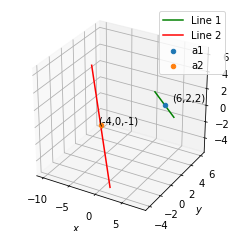
\includegraphics[width=0.6\columnwidth]{p1.png}
    \caption{Skew lines}
    \label{fig:my_label}
\end{figure}
\end{frame}
\begin{frame}{}
    \begin{block}{Finding shortest distance between two skew lines}
Let $\Vec{p_{1}}$, $\Vec{p_{2}}$ be the closest points on lines $L_{1}$ and $L_{2}$ respectively.\\
Then the shortest distance between two skew lines will be the length of line perpendicular to both the lines $L_{1}$, $L_{2}$ and passing through $\Vec{p_{1}}$ and $\Vec{p_{2}}$.\\
The slope of line passing through $\Vec{p_{1}}$ and $\Vec{p_{2}}$ is along $\Vec{p_{2}}-\Vec{p_{1}}$, which is perpendicular to both $L_{1}$ and $L_{2}$. Thus,
\begin{align}
    \label{eq:7}
    \Vec{b_{1}}^\top\brak{\Vec{p_{2}}-\Vec{p_{1}}}={}&0\\
    \label{eq:8}
     \Vec{b_{2}}^\top\brak{\Vec{p_{2}}-\Vec{p_{1}}}={}&0
\end{align}
Let $\Vec{B}=\myvec{\Vec{b_{2}} & \Vec{b}_{1}}$, combining \eqref{eq:7} and \eqref{eq:8} in terms of $\Vec{B}$ and $\Vec{B}^\top$, we have
\begin{align}
    \label{eq:9}
    \Vec{B}^\top\Vec{B}\myvec{\lambda_{2} \\ -\lambda_{1}}= \Vec{B}^\top\brak{\Vec{a}_{1} - \Vec{a}_{2}}
\end{align} 
\end{block}
\end{frame}
\begin{frame}
Substituting values of $a_{1}$, $a_{2}$, $b_{1}$, $b_{2}$, in \eqref{eq:9}
\begin{align}
    \label{eq:10}
    \myvec{17 & 3 \\ 3 & 9}\myvec{\lambda_{2} \\ -\lambda_{1}}=\myvec{20 \\ 12}
\end{align}
Solving for $\lambda_{1}$ and $\lambda_{2}$, 
\begin{align}
    \label{eq:11}
    \myvec{\lambda_{2} \\ -\lambda_{1}}=\myvec{1 \\ 1}
\end{align}
The closest points are
\begin{align}
    \label{eq:12}
    \Vec{p_{1}} &= \myvec{5\\ 4 \\ 0 }   &    \Vec{p_{2}}&=\myvec{ -1\\-2\\-3}
\end{align}
Therefore, the shortest distance between these two skew lines is
\begin{align}
    \label{eq:18}
    d = \norm{\Vec{p_{2}}-\Vec{p_{1}}} = 9
\end{align}
\end{frame}
\begin{frame}{}
    \begin{figure}[htp]
    \centering
    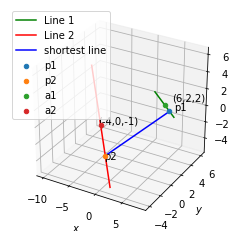
\includegraphics[width=0.6\columnwidth]{p2.png}
    \caption{Plot with points along the least distance}
    \label{fig:my_label}
\end{figure}
\end{frame}
\end{document}
